\documentclass[xcolor={dvipsnames}]{beamer}
\usepackage{color, colortbl}
\usepackage[ngerman,english]{babel}
\usepackage[T1]{fontenc}
\usepackage{lmodern}
\usepackage[compatibility=false]{caption}
\usepackage{subcaption}
\usepackage{tikz}
\usepackage{textgreek}
\usepackage{tabularx}
\usepackage{booktabs}
\usepackage{siunitx}
\usepackage{appendixnumberbeamer}
\usepackage[absolute,overlay]{textpos} %for positioning the logos where I want

\usepackage{animate}
\usepackage{multimedia}
\usepackage{fixltx2e}
\usepackage{multicol}
\usepackage{multirow}
\usepackage{comment}
\DeclareSIUnit\year{yr}

\mode<presentation>
{
  \usetheme{CambridgeUS}     
  \usecolortheme{lily} 
  \definecolor{beamer@violet}{rgb}{0.5,0.3,0.5} % changed this
  \setbeamercolor{structure}{fg=beamer@violet!70!cyan}
  \setbeamercolor{palette primary}{fg=black, bg=gray!30!white!50!cyan!20!}
  \setbeamercolor{palette secondary}{fg=black, bg=gray!30!white!30!cyan!40!}
  \setbeamercolor*{palette tertiary}{bg=gray!20!white!20!cyan!60!}
  
  \setbeamercolor{frametitle}{fg=cyan!60!white!40!,bg=cyan!80!black}
  \setbeamercolor{title}{fg=cyan!80!black}
  \setbeamercolor{normal text}{fg=black,bg=white}
  \setbeamercolor{alerted text}{fg=beamer@violet}
  \setbeamercolor{example text}{fg=beamer@violet!70!cyan}
  
  \usefonttheme{structureitalicserif} 
  \setbeamertemplate{navigation symbols}{}
  \setbeamertemplate{caption}[numbered]
}
\newcommand{\sidlogo}{
  \setlength{\TPHorizModule}{1pt}
  \setlength{\TPVertModule}{1pt}
   % textblock{}{x,y}: pos(x) = rightUpperCorner + (x * \TPHorizModule), pos(y) = leftUpperCorner - (y * \TPVertModule)
  \begin{textblock}{1}(323,12)
   
\includegraphics[width=40pt,height=26pt]{figures/SiD.jpeg}
  \end{textblock}
  } 
\newcommand{\ilclogo}{
  \setlength{\TPHorizModule}{1pt}
  \setlength{\TPVertModule}{1pt}
   % textblock{}{x,y}: pos(x) = rightUpperCorner + (x * \TPHorizModule), pos(y) = leftUpperCorner - (y * \TPVertModule)
  \begin{textblock}{1}(323,12)
   
\includegraphics[width=40pt,height=26pt]{figures/ILC.jpeg}
  \end{textblock}
} 
\newcommand{\flukalogo}{
  \setlength{\TPHorizModule}{1pt}
  \setlength{\TPVertModule}{1pt}
   % textblock{}{x,y}: pos(x) = rightUpperCorner + (x * \TPHorizModule), pos(y) = leftUpperCorner - (y * \TPVertModule)
  \begin{textblock}{1}(315,12)
   
\includegraphics[width=60pt,height=26pt]{figures/fluka_logo.png}
  \end{textblock}
} 

\title[Neutrons from the main beam dumps]{\textbf{\alert{AWLC 2017} \\ \vspace*{0.3cm} The International Linear Collider \\ \LARGE Neutrons from the main beam dumps}}
\author{\textbf{Anne Sch\"utz}}
\institute{\textbf{DESY}}
\date{\textbf{26. June 2017}}

\titlegraphic{
\includegraphics[height=1.0cm]{figures/ILC.jpeg}\hspace*{6cm}~%
   
\includegraphics[height=1.2cm]{figures/DESY_Logo.png}
}

\begin{document}

{
\usebackgroundtemplate{
 \tikz\node[opacity=0.1]{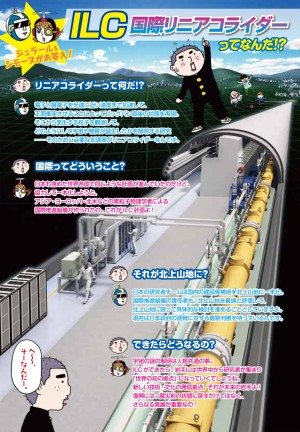
\includegraphics[width=\paperwidth]{figures/Iwatecomics.jpg}};
 % \tikz\node[opacity=0.2]{\centering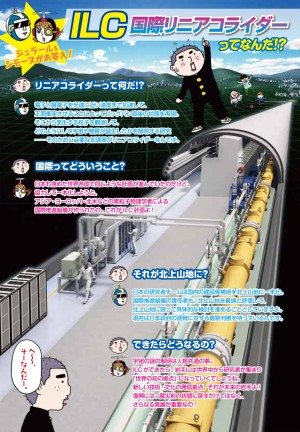
\includegraphics[height=\paperheight]{figures/Iwatecomics.jpg}};
 }
\begin{frame}
  \titlepage
\end{frame}
}

\begin{frame}{Table of contents}
  \tableofcontents
\end{frame}



\section{FLUKA simulation of the ILC Beam Dump}
\subsection{Project Overview}
{
\usebackgroundtemplate{
\vbox to \paperheight{\vfil
 \tikz\node[opacity=0.1]{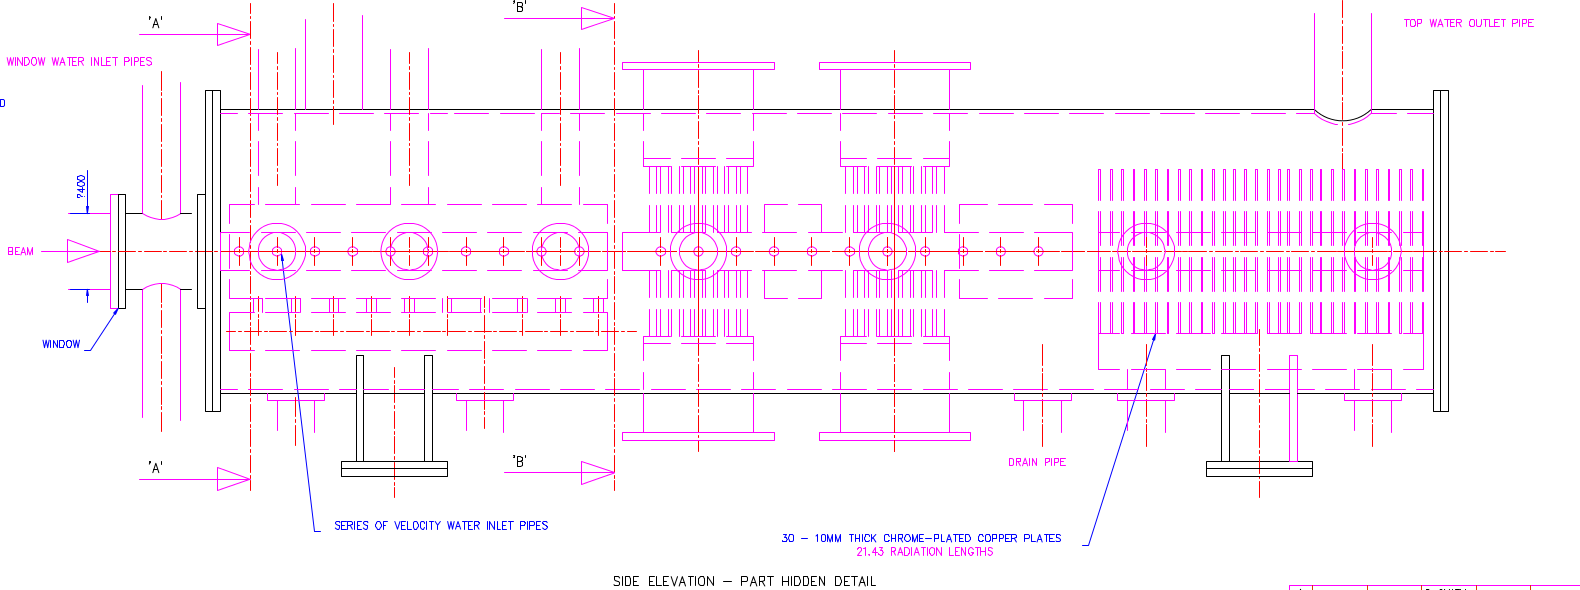
\includegraphics[width=\paperwidth]{figures/TB-0067-300-00-A_yz_view.png}};
 \vfil}
}
\begin{frame}{Neutron Background and Beam Dump Irradiation}
\flukalogo
The 17\,MW\footnote{13.7\,MW average beam power + 20\% margin} beam is dumped into a water tank after collision.\\The activation of the dump surrounding will permit access to the dump area. Neutrons ($\lesssim$\SI{e10}{\per\square\centi\metre\per\year}) are emitted that irradiate the surroundings, and travel back towards the detectors.\\
\alert{Project goal: Simulating the energy depostion, irradiation, and background particles:}
\begin{enumerate}
 \item Simulating the acitvation, and the neutrons from the beam dump with FLUKA, using the design drawings by B. Smith~\cite{Smith} to model the dump and the surrounding.
 \item Neutrons through the EXT line:\\
 With Benno List (DESY): Python program to plug the real extraction line lattice into FLUKA. Realistic simulation of the interaction between the neutrons and the lattice.
 \item Simulating the neutrons reaching the interaction point in a full detector simulation.
\end{enumerate}
\end{frame}
}

\AtBeginSubsection[] {
  \begin{frame}<beamer>
     \tableofcontents[currentsection,
     currentsubsection,
     %hideothersubsections,
     subsectionstyle=show/shaded/hide,
     subsubsectionstyle=show/show/hide]
  \end{frame}
}

\subsection{The Beam Dump Designs}
\begin{frame}{Designs by B. Smith}
Design drawings by B. Smith, 2006-2007~\cite{Smith}:
\begin{itemize}
 \item two different designs for the water beam dump: 0-TB-0067-210-00-A, 0-TB-0067-300-00-A
 \item shielding walls: 0-TB-0067-404-00-A
 \item surface site: 0-TB-0067-410-00-A
\end{itemize}
Report ``18\,MW Water Beam Dump Design''~\cite{Smith_Report} about considerations and studies of:
\begin{itemize}
 \item Material qualities
 \item Water temperature and pressure
 \item Technical specifications of the dump designs
\end{itemize}
\end{frame}

\begin{frame}{\textbf{Surface site}: 0-TB-0067-410-00-A}
\centering
\only<1>{
  \includegraphics[width=0.9\textwidth]{figures/0067_404-House.png}
 }
 \only<2>{
   \includegraphics[height=0.92\textheight]{figures/0067_404-House_zoom.png}
 }
\end{frame}
\begin{frame}{\textbf{Shielding walls}: 0-TB-0067-404-00-A}
\centering
\only<1>{
 \includegraphics[width=0.92\textwidth]{figures/0067_404-Shielding.png}
 }
 \only<2>{
  \includegraphics[width=0.65\textwidth,angle=90]{figures/0067_404-Shielding_zoom.png}
  }
\end{frame}

\begin{frame}{\textbf{Design 1}: 0-TB-0067-210-00-A}
\centering
 \includegraphics[width=0.92\textwidth]{figures/TB-0067-210-00-A.png}
\end{frame}
{
\usebackgroundtemplate{
\vbox to \paperheight{\vspace*{1.2cm}
 \tikz\node[opacity=0.3]{\hspace*{0.6cm} \includegraphics[width=0.92\textwidth]{figures/TB-0067-210-00-A.png}};
 \vfil}}
\begin{frame}{\textbf{Design 1}: 0-TB-0067-210-00-A}
\begin{columns}
 \begin{column}{0.5\textwidth}
  Vessel:
  \begin{itemize}
   \item Diameter: 1.5\,m
   \item Length: 6.5\,m
   \item 316L Stainless Steel
   \item Water pressure: 10\,bar
  \end{itemize}
  Window:
  \begin{itemize}
   \item Diameter: 300\,mm
   \item Thickness: 1\,mm
   \item Titanium alloy: Ti-6Al-4V 
  \end{itemize}
 \end{column}
 \begin{column}{0.5\textwidth}
  27\,X\textsubscript{0} needed to stop a 500\,GeV beam:
  \begin{itemize}
   \item Water: 18\,X\textsubscript{0}
   \item Water cooled copper plates: 9\,X\textsubscript{0} = 126\,mm
  \end{itemize}  
 \end{column}
\end{columns}

\end{frame}
}
\begin{frame}{\textbf{Design 1}: 0-TB-0067-210-00-A}
\centering
 \includegraphics[width=\textwidth]{figures/Design1_geometry.png}
\end{frame}
\begin{frame}{\textbf{Design 1}: 0-TB-0067-210-00-A}
\centering
 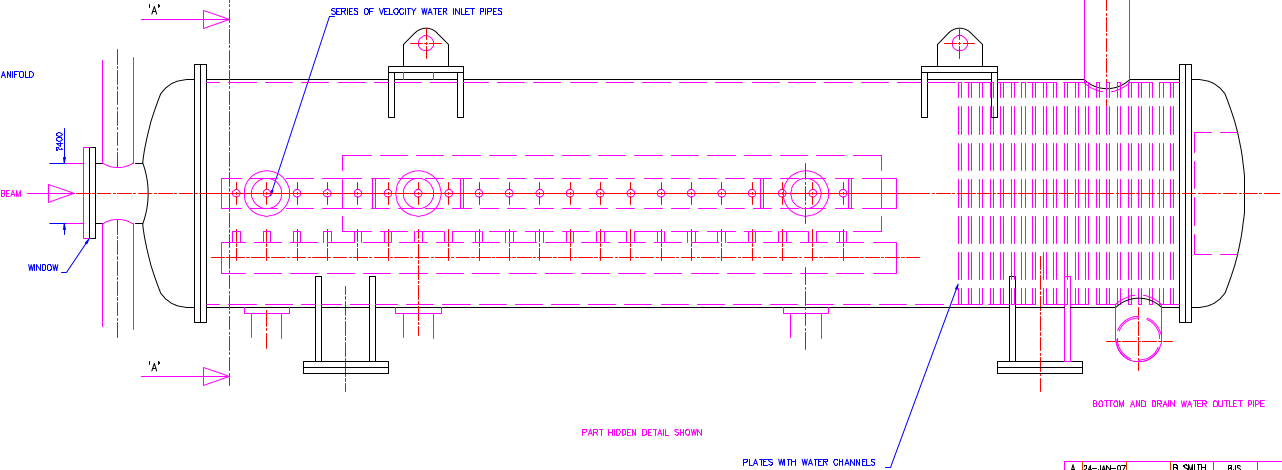
\includegraphics[width=0.5\textwidth]{figures/TB-0067-210-00-A_yz_view.png}
 \hfill
 \includegraphics[width=0.48\textwidth]{figures/Design1_geometry_3Dinside.png}
\end{frame}

\begin{frame}{\textbf{Design 2}: 0-TB-0067-300-00-A}
\centering
  \includegraphics[width=0.92\textwidth]{figures/TB-0067-300-00-A.png}
\end{frame}
{
\usebackgroundtemplate{
\vbox to \paperheight{\vspace*{1.2cm}
 \tikz\node[opacity=0.3]{\hspace*{0.6cm} \includegraphics[width=0.92\textwidth]{figures/TB-0067-300-00-A.png}};
 \vfil}}
\begin{frame}{\textbf{Design 2}: 0-TB-0067-210-00-A}
\begin{columns}
 \begin{column}{0.5\textwidth}
  Vessel:
  \begin{itemize}
   \item Diameter: 1.5\,m
   \item Length: 6.5\,m
   \item 316L Stainless Steel
   \item Water pressure: 10\,bar
  \end{itemize}
  Window:
  \begin{itemize}
   \item Diameter: 300\,mm
   \item Thickness: 1\,mm
   \item Titanium alloy: Ti-6Al-4V 
  \end{itemize}
 \end{column}
 \begin{column}{0.5\textwidth}
  27\,X\textsubscript{0} needed to stop a 500\,GeV beam:
  \begin{itemize}
   \item Water: 18\,X\textsubscript{0}
   \item Water cooled copper plates: 9\,X\textsubscript{0} = 126\,mm
  \end{itemize}  
    Additionally high water pressure section:
  \begin{itemize}
   \item Titanium tubes
   \item High pressure water flow
   \item In total 1.98\,X\textsubscript{0}
  \end{itemize} 
 \end{column}
\end{columns}

\end{frame}
}
\begin{frame}{\textbf{Design 2}: 0-TB-0067-300-00-A}
\centering
  \includegraphics[width=\textwidth]{figures/Design2_geometry.png}
\end{frame}
\begin{frame}{\textbf{Design 2}: 0-TB-0067-300-00-A}
\centering
  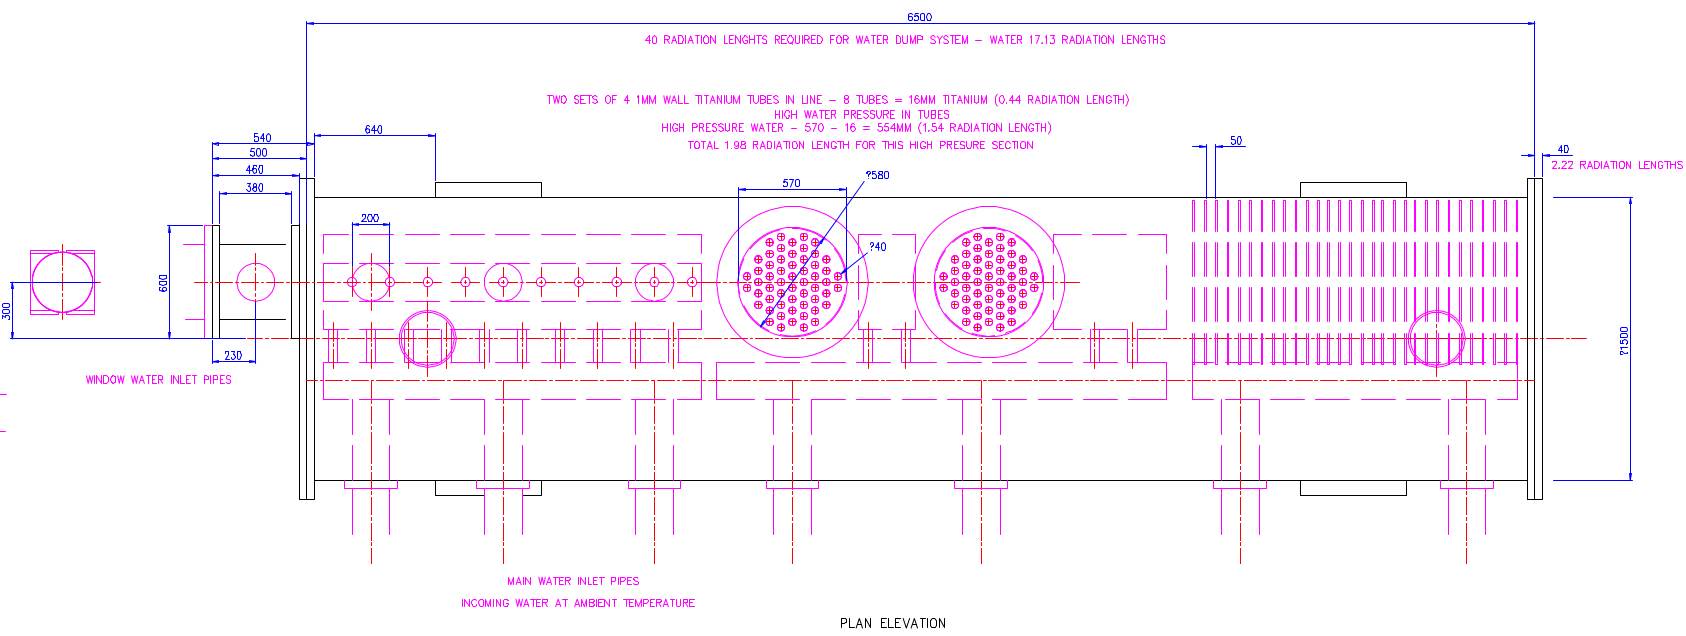
\includegraphics[width=0.5\textwidth]{figures/TB-0067-300-00-A_xz_view.png}
  \hfill
  \includegraphics[width=0.48\textwidth]{figures/Design2_geometry_drawing_xz.png}
\end{frame}
\begin{frame}{\textbf{Design 2}: 0-TB-0067-300-00-A}
\centering
  \includegraphics[width=0.49\textwidth]{figures/Design2_geometry_3Dinside1.png}
    \includegraphics[width=0.49\textwidth]{figures/Design2_geometry_3Dinside2.png}\\
      \includegraphics[width=0.49\textwidth]{figures/Design2_geometry_3Dinside3.png}
\end{frame}



\subsection{The FLUKA simulation}
\begin{frame}
 ILC1000B:
 \begin{itemize}
  \item Beam energy: 500\,GeV
  \item Bunch population: 1.74e10
  \item Bunch size: \textsigma\textsubscript{x} = 2.4\,mm, \textsigma\textsubscript{y} = 0.22\,mm
  \item Bunches per train: 2450
  \item Bunch train duration: 896.7\,\textmu s
 \end{itemize}

Beams are considered un-collided and un-disrupted.
\end{frame}


\subsubsection{Deposited Energy and Dose}
\begin{frame}{Deposited Energy}
\begin{center}
\hspace*{1.6cm} Design 1 \hfill Design 2 \hspace*{1.8cm} \\
  \includegraphics[width=0.52\textwidth]{figures/Energy_deposition_xz_Design1.pdf}
    \includegraphics[width=0.52\textwidth]{figures/Energy_deposition_xz_Design2.pdf}
\end{center}
 Shielding walls seem to stop particles fluxes well, but large scattering in Design 2 at high water pressure sections.
\end{frame}
\begin{frame}{Maximum Deposited Engery over Z}
\begin{center}
\hspace*{1.6cm} Design 1 \hfill Design 2 \hspace*{1.8cm} \\
  \includegraphics[width=0.51\textwidth]{figures/Energy_deposition_1DMax_z_Design1.pdf}
    \includegraphics[width=0.51\textwidth]{figures/Energy_deposition_1DMax_z_Design2.pdf}
\end{center}
  Maximum deposited energy within the water tank up to \textbf{10\textsuperscript{8}-10\textsuperscript{9}\,GeV/cm\textsuperscript{3} (= 0.016 - 0.16 J/cm\textsuperscript{3}) per bunch}.
\end{frame}
\begin{frame}{Average Deposited Energy and Power per bunch}
\begin{center}
\begin{tabular}{cc|c|c|c|c|c|c|c|}
\cline{3-5}
& & \textbf{Water} & \textbf{Vessel} & \textbf{Window} \\
\hline
\multicolumn{1}{ |c| }{\multirow{2}{*}{Design 1}}& 
  \multicolumn{1}{ |c| }{Dep. Energy [J/cm\textsuperscript{3}]} & 233.24 & 5.14 & 0.0019\\
\cline{2-5}
\multicolumn{1}{ |c| }{} & \multicolumn{1}{ |c| }{Power [kW/cm\textsuperscript{3}]} & 260.1 & 5.728  & 0.002\\
\hline
\hline
\multicolumn{1}{ |c| }{\multirow{2}{*}{Design 2}}& 
  \multicolumn{1}{ |c| }{Dep. Energy [J/cm\textsuperscript{3}]} & 240.67 & 4.36 & 0.0018\\
\cline{2-5}
\multicolumn{1}{ |c| }{} & \multicolumn{1}{ |c| }{Power [kW/cm\textsuperscript{3}]} & 268.4 & 4.866 & 0.002\\
\hline
\end{tabular}
\vspace*{1cm}\\
\begin{tabular}{cc|c|c|c|}
\cline{3-5}
& & \textbf{Cu plate 1} & \textbf{Last Cu plate} & \textbf{Iron shielding}\\
\hline
\multicolumn{1}{ |c| }{\multirow{2}{*}{Design 1}}& 
  \multicolumn{1}{ |c| }{[J/cm\textsuperscript{3}]} & 4.44 & 1.46 & 5.09\\
\cline{2-5}
\multicolumn{1}{ |c| }{} & \multicolumn{1}{ |c| }{ [kW/cm\textsuperscript{3}]} & 4.935 & 0.256 & 5.685\\
\hline
\hline
\multicolumn{1}{ |c| }{\multirow{2}{*}{Design 2}}& 
  \multicolumn{1}{ |c| }{[J/cm\textsuperscript{3}]} & 1.58 & 0.13 & 5.87\\
\cline{2-5}
\multicolumn{1}{ |c| }{} & \multicolumn{1}{ |c| }{[kW/cm\textsuperscript{3}]} & 1.760 & 0.141 & 6.541\\
\hline
\end{tabular}
\end{center}
\end{frame}

\begin{frame}{Instantanuous Dose Equivalent}
\begin{center}
\hspace*{1.8cm} Design 1 \hfill Design 2 \hspace*{1.8cm} \\
  \includegraphics[width=0.52\textwidth]{figures/Dose_equivalent_total_Design1.pdf}
    \includegraphics[width=0.52\textwidth]{figures/Dose_equivalent_total_Design2.pdf}
\end{center}
\end{frame}
\begin{frame}{Maximum Instantanuous Dose Equivalent over Z}
\begin{center}
\hspace*{1.8cm} Design 1 \hfill Design 2 \hspace*{1.8cm} \\
  \includegraphics[width=0.51\textwidth]{figures/Dose_equivalent_total_1DMax_z_Design1.pdf}
    \includegraphics[width=0.51\textwidth]{figures/Dose_equivalent_total_1DMax_z_Design2.pdf}
\end{center}
Maximum dose equivalent within the water tank up to \textbf{100\,Sv per bunch}.
\end{frame}
\begin{frame}{Dose equivalent after cooling times}
\textbf{After one month of beam operation}, the beam is turned off.\\
Different \textbf{cooling times} are considered:\\
\textbf{1 minute, 1 hour, 1 day, 1 month, and 1 year}\\
\hspace*{1.6cm} Design 1 \hfill Design 2 \hspace*{1.8cm} \\
  \begin{center}
  \animategraphics[loop,width=0.49\textwidth]{0.5}{DoseEQ_Time/Design1_}{1}{5}
  \animategraphics[loop,width=0.49\textwidth]{0.5}{DoseEQ_Time/Design2_}{1}{5}
  \end{center}
\end{frame}
\begin{frame}
  \frametitle{Dose equivalent after cooling times - Design 1}
  \hypertarget{coolingtimesprev_Design1}{}
  \centering
    \hspace*{1.2cm} Instantanuous \hfill After 1 minute \hfill After 1 hour \hspace*{1.5cm} \\
  \hyperlink{Dose_equivalent_Design1}{\includegraphics[width=0.3\textwidth]{figures/Dose_equivalent_total_Design1.pdf}}
  \hyperlink{Dose_equivalent_minute_Design1}{\includegraphics[width=0.3\textwidth]{DoseEQ_Time/Design1_1.pdf}}
  \hyperlink{Dose_equivalent_hour_Design1}{\includegraphics[width=0.3\textwidth]{DoseEQ_Time/Design1_2.pdf}}\\
    \hspace*{1.2cm} After 1 day \hfill After 1 month \hfill After 1 year\hspace*{1.5cm} \\
  \hyperlink{Dose_equivalent_day_Design1}{\includegraphics[width=0.3\textwidth]{DoseEQ_Time/Design1_3.pdf}}
  \hyperlink{Dose_equivalent_month_Design1}{\includegraphics[width=0.3\textwidth]{DoseEQ_Time/Design1_4.pdf}}
  \hyperlink{Dose_equivalent_year_Design1}{\includegraphics[width=0.3\textwidth]{DoseEQ_Time/Design1_5.pdf}}
\end{frame}
\begin{frame}
  \frametitle{Dose equivalent after cooling times - Design 2}
  \hypertarget{coolingtimesprev_Design2}{}
  \centering
    \hspace*{1.2cm} Instantanuous \hfill After 1 minute \hfill After 1 hour \hspace*{1.5cm} \\
  \hyperlink{Dose_equivalent_Design2}{\includegraphics[width=0.3\textwidth]{figures/Dose_equivalent_total_Design2.pdf}}
  \hyperlink{Dose_equivalent_minute_Design2}{\includegraphics[width=0.3\textwidth]{DoseEQ_Time/Design2_1.pdf}}
  \hyperlink{Dose_equivalent_hour_Design2}{\includegraphics[width=0.3\textwidth]{DoseEQ_Time/Design2_2.pdf}}\\
    \hspace*{1.2cm} After 1 day \hfill After 1 month \hfill After 1 year\hspace*{1.5cm} \\
  \hyperlink{Dose_equivalent_day_Design2}{\includegraphics[width=0.3\textwidth]{DoseEQ_Time/Design2_3.pdf}}
  \hyperlink{Dose_equivalent_month_Design2}{\includegraphics[width=0.3\textwidth]{DoseEQ_Time/Design2_4.pdf}}
  \hyperlink{Dose_equivalent_year_Design2}{\includegraphics[width=0.3\textwidth]{DoseEQ_Time/Design2_5.pdf}}
\end{frame}
\begin{frame}{Dose Equivalent over Time}
\centering
  \includegraphics[width=0.52\textwidth]{figures/DoseEQ_Time_Comparison.png}\\
\textbf{After one year}, the dose rate drops to \textbf{}.
\end{frame}

\AtBeginSubsubsection[] {
  \begin{frame}<beamer>
     \tableofcontents[currentsection,
     currentsubsection,
     %hideothersubsections,
     subsectionstyle=show/shaded/hide,
     subsubsectionstyle=show/show/hide]
  \end{frame}
}

\subsubsection{Residual nuclei}
\begin{frame}{Residual nuclei after cooling times}
\textbf{After one month of beam operation}, the beam is turned off.\\
Different \textbf{cooling times} are considered:\\
\textbf{1 minute, 1 hour, 1 day, 1 month, and 1 year}
  \begin{center}
  \hspace*{1.6cm} Design 1 \hfill Design 2 \hspace*{1.8cm} \\
  \animategraphics[loop,width=0.49\textwidth]{0.5}{Residual_Time/Design1_}{1}{5}
  \animategraphics[loop,width=0.49\textwidth]{0.5}{Residual_Time/Design2_}{1}{5}
  \end{center}
\end{frame}
\begin{frame}
  \frametitle{Residual nuclei after cooling times - Design 1}
  \hypertarget{residualtimesprev_Design1}{}
  \centering
    \hspace*{1.6cm} Instantanuous \hfill After 1 minute \hfill After 1 hour \hspace*{1.8cm} \\
  \hyperlink{Residual_nuclei_Design1}{\includegraphics[width=0.3\textwidth]{figures/Residual_nuclei_Design1.pdf}}
  \hyperlink{Residual_nuclei_minute_Design1}{\includegraphics[width=0.3\textwidth]{Residual_Time/Design1_1.pdf}}
  \hyperlink{Residual_nuclei_hour_Design1}{\includegraphics[width=0.3\textwidth]{Residual_Time/Design1_2.pdf}}\\
    \hspace*{1.6cm} After 1 day \hfill After 1 month \hfill After 1 year\hspace*{1.8cm} \\
  \hyperlink{Residual_nuclei_day_Design1}{\includegraphics[width=0.3\textwidth]{Residual_Time/Design1_3.pdf}}
  \hyperlink{Residual_nuclei_month_Design1}{\includegraphics[width=0.3\textwidth]{Residual_Time/Design1_4.pdf}}
  \hyperlink{Residual_nuclei_year_Design1}{\includegraphics[width=0.3\textwidth]{Residual_Time/Design1_5.pdf}}
\end{frame}
\begin{frame}
  \frametitle{Residual nuclei after cooling times - Design 2}
  \hypertarget{residualtimesprev_Design2}{}
  \centering
    \hspace*{1.6cm} Instantanuous \hfill After 1 minute \hfill After 1 hour \hspace*{1.8cm} \\
  \hyperlink{Residual_nuclei_Design2}{\includegraphics[width=0.3\textwidth]{figures/Residual_nuclei_Design2.pdf}}
  \hyperlink{Residual_nuclei_minute_Design2}{\includegraphics[width=0.3\textwidth]{Residual_Time/Design2_1.pdf}}
  \hyperlink{Residual_nuclei_hour_Design2}{\includegraphics[width=0.3\textwidth]{Residual_Time/Design2_2.pdf}}\\
    \hspace*{1.6cm} After 1 day \hfill After 1 month \hfill After 1 year\hspace*{1.8cm} \\
  \hyperlink{Residual_nuclei_day_Design2}{\includegraphics[width=0.3\textwidth]{Residual_Time/Design2_3.pdf}}
  \hyperlink{Residual_nuclei_month_Design2}{\includegraphics[width=0.3\textwidth]{Residual_Time/Design2_4.pdf}}
  \hyperlink{Residual_nuclei_year_Design2}{\includegraphics[width=0.3\textwidth]{Residual_Time/Design2_5.pdf}}
\end{frame}

\begin{frame}{Number of radio-nuclides}
\begin{center}
\begin{tabular}{|c|c|c|c|}
\hline
 & Tritium & Berillyum & ... \\
\hline
Design 1 & 1 & 2 & 3\\
\hline
\hline
Design 2 & 1 & 2 & 3\\
\hline
\end{tabular}
\end{center}

\centering
\hspace*{1.6cm} Tritium flux: Design 1 \hfill Tritium flux: Design 2 \hspace*{1.8cm} \\
  \includegraphics[width=0.52\textwidth]{figures/Tritium_flux_xz_Design1.pdf}
    \includegraphics[width=0.52\textwidth]{figures/Tritium_flux_xz_Design2.pdf}
\end{frame}

\subsubsection{Particle Fluxes}

\begin{frame}{Electron and Photon fluxes from one bunch}
\centering
Design 1 \hspace*{1.4cm} Electrons \hfill Photons \hspace*{3.1cm} \\
 \includegraphics[width=0.37\textwidth]{figures/Electron_flux_xz_Design1.pdf}
  \includegraphics[width=0.37\textwidth]{figures/Photon_flux_xz_Design1.pdf}\\
Design 2 \hspace*{1.4cm} Electrons \hfill Photons \hspace*{3.1cm} \\ 
\includegraphics[width=0.37\textwidth]{figures/Electron_flux_xz_Design2.pdf}
  \includegraphics[width=0.37\textwidth]{figures/Photon_flux_xz_Design2.pdf}
\end{frame}
\begin{frame}{Neutron fluxes from one bunch: \textbf{Design 1}}
\begin{columns}
 \begin{column}{0.5\textwidth}
    \includegraphics[width=\textwidth]{figures/Neutron_flux_xz_Design1.pdf}
 \end{column}
 \begin{column}{0.5\textwidth}
  The neutrons spread more in the positive x and y-direction. Within the tank, the neutrons are mainly produced in the water vortex system. When the beam is stopped by the copper plates, the neutron production rate decreases.
 \end{column}
\end{columns}
  \centering
\hspace*{1cm} x-direction \hfill y-direction \hfill z-direction \hspace*{1cm} \\
  \includegraphics[width=0.31\textwidth]{figures/Neutron_flux_1DMax_x_Design1.pdf}\hfill
  \includegraphics[width=0.31\textwidth]{figures/Neutron_flux_1DMax_y_Design1.pdf}\hfill
  \includegraphics[width=0.31\textwidth]{figures/Neutron_flux_1DMax_z_Design1.pdf}
\end{frame}
\begin{frame}{Neutron fluxes from one bunch: \textbf{Design 2}}
\begin{columns}
 \begin{column}{0.5\textwidth}
    \includegraphics[width=\textwidth]{figures/Neutron_flux_xz_Design2.pdf}
 \end{column}
 \begin{column}{0.5\textwidth}
  The neutrons again spread more in the positive x and y-direction. Within the tank, the point of highest neutron production is the high pressure water system. The production rate again decreases with the beam being stopped by the copper plates.
 \end{column}
\end{columns}
  \centering
\hspace*{1cm} x-direction \hfill y-direction \hfill z-direction \hspace*{1cm} \\
  \includegraphics[width=0.31\textwidth]{figures/Neutron_flux_1DMax_x_Design2.pdf}\hfill
  \includegraphics[width=0.31\textwidth]{figures/Neutron_flux_1DMax_y_Design2.pdf}\hfill
  \includegraphics[width=0.31\textwidth]{figures/Neutron_flux_1DMax_z_Design2.pdf}
\end{frame}


\section{Summary and Outlook}
\begin{frame}{Summary and outlook}
 \flukalogo
 Aspects already addressed:
\begin{itemize}
 \item The dose of the beam dump surrounding,
 \item the number of particles, such as neutrons, produced,
 \item the amount of tritium produced in the water,
 \item the effect of the beam dump design.
\end{itemize}
\vspace*{0.2cm}
 Goals for the next months:
\begin{itemize}
 \item Studying the influence of the water composition (amount of deuterium),
  \item the influence of the steel composition of the tank container,
 \item simulating the neutron flux through the EXT line,
 \item the number of neutrons reaching the IP,
 \item the neutron occupancy in SiD.
\end{itemize}
\end{frame}


\section*{The end}
{
\usebackgroundtemplate{
 \tikz\node[opacity=0.1]{\includegraphics[width=\paperwidth,resolution=200]{figures/ilc-Comic.png}};
 % \tikz\node[opacity=0.2]{\centering\includegraphics[height=\paperheight]{figures/Iwatecomics.jpg}};
 }
\begin{frame}
\ilclogo
\begin{center}
\textcolor{RubineRed}{
	\LARGE Thanks!\\
}
\end{center}
\end{frame}
}

\section*{References}
\begin{thebibliography}{9}
\begin{frame}{References}
\setbeamertemplate{bibliography item}[text]
\bibitem{Smith} B. Smith (Rutherford Lab), \emph{Design drawings 0-TB-0067-300-00-A, 0-TB-0067-210-00-A, 0-TB-0067-404-00-A}, Dec. 2006 - Jan. 2007
\bibitem{TDR} T. Behnke, et al.
\emph{The International Linear Collider - Technical Design Report}, 2013.
\bibitem{LHC TDR} \emph{LHC - Design Report}, \url{http://ab-div.web.cern.ch/ab-div/Publications/LHC-DesignReport.html}
\bibitem{IP beam parameters} ATLAS-CONF-2010-027. \emph{Characterization of Interaction-Point Beam Parameters Using the pp Event-Vertex Distribution Reconstructed in the ATLAS Detector at the LHC}, 2010. \url{http://cds.cern.ch/record/1277659/files/ATLAS-CONF-2010-027.pdf}
\end{frame}
\end{thebibliography}

%--------------------------------------------------------------------------------
\appendix

\begin{frame}
\begin{center}
\LARGE Additional Material
\end{center}
  \tableofcontents
\end{frame}

\section{FLUKA simulation}
\subsection{Particle Fluxes}
\begin{frame}{Proton fluxes}
\centering
\hspace*{2cm} Design 1 \hfill Design 2 \hspace*{2cm} \\
  \includegraphics[width=0.52\textwidth]{figures/Proton_flux_xz_Design1.pdf}
    \includegraphics[width=0.52\textwidth]{figures/Proton_flux_xz_Design2.pdf}
\end{frame}

\section{ILC}

%------Definition for column color in table
\definecolor{Gray}{gray}{0.9}
\newcolumntype{g}{>{\columncolor{Gray}}r}
%-----------------------------------------
\subsection{The ILC beam parameters}
\begin{frame}{The beam parameters of the ILC compared to LHC}
\ilclogo

\begin{table}[]
\centering
\begin{tabularx}{\textwidth}{ll|rrrg}
\hline
& & \multicolumn{1}{>{\centering}p{1.5cm}}{\textbf{Baseline 500}} & \multicolumn{1}{>{\centering}p{1.5cm}}{\textbf{Lumi Upgrade}} & \multicolumn{1}{>{\centering}p{1.5cm}}{\textbf{TeV Upgrade}} & {\centering\textbf{LHC 25ns}} \\ 
\hline
\cline{1-6}
\hline
E$_{CM}$  &[\si{\GeV}] & 500  & 500  & \num{1000} & \num{14000}\\
n$_b$ & & \num{1312} & \num{2625} & \num{2450} &  \num{2808} \\
$\Delta t_b$ &[\si{\nano\second}] & 554  & 366   & 366 & 25 \\
N & & \num{2.0e10}  & \num{2.0e10}  & \num{1.74e10}  & \num{11.5e10}\\
q$_b$ &[\si{\nano\coulomb}] & 3.2  & 3.2  &  2.7 & 18.4 \\
$\sigma_x^*$ &[\si{\nano\metre}] & 474  & 474  &  481 & \num{16700}\\
$\sigma_y^*$ &[\si{\nano\metre}] & 5.9 &  5.9  &  2.8 & \num{16700}\\
$\sigma_z$ &[\si{\milli\metre}] & 0.3  &  0.3  &  0.25 & 0.755\\
L &[\si{\per\centi\metre\squared\per\second}] & \num{1.8e34} & \num{3.6e34} & \num{3.6e34} & \num{1.0e34}\\
\hline
\end{tabularx}
\end{table}
\end{frame}

\begin{frame}{ILC baseline parameters}
\ilclogo
\centering
	\includegraphics[width=\textwidth]{figures/ILCTDR-VOLUME_3-PART_II_ILCparameters.pdf}
\end{frame}
\begin{frame}{ILC parameters for the different upgrade stages}
\ilclogo
\centering
	\includegraphics[width=0.8\textwidth]{figures/ILCTDR-VOLUME_3-PART_II_ILCparametersUpgrades.pdf}
\end{frame}

\section{Zoom Plots}
\begin{frame}
  \begin{center}
    \huge
    ZOOM PLOTS\\
    \tiny
    Here be dragons
  \end{center}
\end{frame}
\begin{frame}[plain]
 \hypertarget{Dose_equivalent_Design1}{\hyperlink{coolingtimesprev_Design1}{\includegraphics[width=\textwidth]{figures/Dose_equivalent_total_Design1.pdf}}}
\end{frame}
\begin{frame}[plain]
 \hypertarget{Dose_equivalent_minute_Design1}{\hyperlink{coolingtimesprev_Design1}{\includegraphics[width=\textwidth]{DoseEQ_Time/Design1_1.pdf}}}
\end{frame}
\begin{frame}[plain]
 \hypertarget{Dose_equivalent_hour_Design1}{\hyperlink{coolingtimesprev_Design1}{\includegraphics[width=\textwidth]{DoseEQ_Time/Design1_2.pdf}}}
\end{frame}
\begin{frame}[plain]
 \hypertarget{Dose_equivalent_day_Design1}{\hyperlink{coolingtimesprev_Design1}{\includegraphics[width=\textwidth]{DoseEQ_Time/Design1_3.pdf}}}
\end{frame}
\begin{frame}[plain]
 \hypertarget{Dose_equivalent_month_Design1}{\hyperlink{coolingtimesprev_Design1}{\includegraphics[width=\textwidth]{DoseEQ_Time/Design1_4.pdf}}}
\end{frame}
\begin{frame}[plain]
 \hypertarget{Dose_equivalent_year_Design1}{\hyperlink{coolingtimesprev_Design1}{\includegraphics[width=\textwidth]{DoseEQ_Time/Design1_5.pdf}}}
\end{frame}
%------------------------------------
\begin{frame}[plain]
 \hypertarget{Dose_equivalent_Design2}{\hyperlink{coolingtimesprev_Design2}{\includegraphics[width=\textwidth]{figures/Dose_equivalent_total_Design2.pdf}}}
\end{frame}
\begin{frame}[plain]
 \hypertarget{Dose_equivalent_minute_Design2}{\hyperlink{coolingtimesprev_Design2}{\includegraphics[width=\textwidth]{DoseEQ_Time/Design2_1.pdf}}}
\end{frame}
\begin{frame}[plain]
 \hypertarget{Dose_equivalent_hour_Design2}{\hyperlink{coolingtimesprev_Design2}{\includegraphics[width=\textwidth]{DoseEQ_Time/Design2_2.pdf}}}
\end{frame}
\begin{frame}[plain]
 \hypertarget{Dose_equivalent_day_Design2}{\hyperlink{coolingtimesprev_Design2}{\includegraphics[width=\textwidth]{DoseEQ_Time/Design2_3.pdf}}}
\end{frame}
\begin{frame}[plain]
 \hypertarget{Dose_equivalent_month_Design2}{\hyperlink{coolingtimesprev_Design2}{\includegraphics[width=\textwidth]{DoseEQ_Time/Design2_4.pdf}}}
\end{frame}
\begin{frame}[plain]
 \hypertarget{Dose_equivalent_year_Design2}{\hyperlink{coolingtimesprev_Design2}{\includegraphics[width=\textwidth]{DoseEQ_Time/Design2_5.pdf}}}
\end{frame}
%------------------------------------
\begin{frame}[plain]
 \hypertarget{Residual_nuclei_Design1}{\hyperlink{residualtimesprev_Design1}{\includegraphics[width=\textwidth]{figures/Residual_nuclei_Design1.pdf}}}
\end{frame}
\begin{frame}[plain]
 \hypertarget{Residual_nuclei_minute_Design1}{\hyperlink{residualtimesprev_Design1}{\includegraphics[width=\textwidth]{Residual_Time/Design1_1.pdf}}}
\end{frame}
\begin{frame}[plain]
 \hypertarget{Residual_nuclei_hour_Design1}{\hyperlink{residualtimesprev_Design1}{\includegraphics[width=\textwidth]{Residual_Time/Design1_2.pdf}}}
\end{frame}
\begin{frame}[plain]
 \hypertarget{Residual_nuclei_day_Design1}{\hyperlink{residualtimesprev_Design1}{\includegraphics[width=\textwidth]{Residual_Time/Design1_3.pdf}}}
\end{frame}
\begin{frame}[plain]
 \hypertarget{Residual_nuclei_month_Design1}{\hyperlink{residualtimesprev_Design1}{\includegraphics[width=\textwidth]{Residual_Time/Design1_4.pdf}}}
\end{frame}
\begin{frame}[plain]
 \hypertarget{Residual_nuclei_year_Design1}{\hyperlink{residualtimesprev_Design1}{\includegraphics[width=\textwidth]{Residual_Time/Design1_5.pdf}}}
\end{frame}
%------------------------------------
\begin{frame}[plain]
 \hypertarget{Residual_nuclei_Design2}{\hyperlink{residualtimesprev_Design2}{\includegraphics[width=\textwidth]{figures/Residual_nuclei_Design2.pdf}}}
\end{frame}
\begin{frame}[plain]
 \hypertarget{Residual_nuclei_minute_Design2}{\hyperlink{residualtimesprev_Design2}{\includegraphics[width=\textwidth]{Residual_Time/Design2_1.pdf}}}
\end{frame}
\begin{frame}[plain]
 \hypertarget{Residual_nuclei_hour_Design2}{\hyperlink{residualtimesprev_Design2}{\includegraphics[width=\textwidth]{Residual_Time/Design2_2.pdf}}}
\end{frame}
\begin{frame}[plain]
 \hypertarget{Residual_nuclei_day_Design2}{\hyperlink{residualtimesprev_Design2}{\includegraphics[width=\textwidth]{Residual_Time/Design2_3.pdf}}}
\end{frame}
\begin{frame}[plain]
 \hypertarget{Residual_nuclei_month_Design2}{\hyperlink{residualtimesprev_Design2}{\includegraphics[width=\textwidth]{Residual_Time/Design2_4.pdf}}}
\end{frame}
\begin{frame}[plain]
 \hypertarget{Residual_nuclei_year_Design2}{\hyperlink{residualtimesprev_Design2}{\includegraphics[width=\textwidth]{Residual_Time/Design2_5.pdf}}}
\end{frame}
\end{document}
